\subsection{Crowdfunding}
El financiamiento colectivo o crowdfunding es un sistema que, utilizando internet como base de operaciones, busca generar una respuesta económica activa en el usuario \parencite{cr_lopezgolan2017crowdfunding}.

Combinando ideas de microfinanzas y crowdsourcing, el crowdfunding es la práctica de financiar una empresa o un proyecto al recaudar muchas pequeñas cantidades de dinero de un gran número de personas. Este mecanismo de financiamiento ha sido recibido por los recaudadores de fondos, el público en general y los formuladores de políticas. La industria de crowdfunding ha crecido rápidamente en los últimos años, así como el crecimiento exponencial del número de plataformas de crowdfunding, el número de proyectos expuestos allí y el número de capital total recaudado en esos sitios web \parencite{cr_xuefeng2018chcrowdplatf}.

La cantidad de grupos de crowdfunding varía según distintos autores. Según \citeauthor{cr_hollas2013crwd}, se clasifican en 4 modelos: basado en donaciones, recompensas, capital y deuda. \citeauthor{cr_colgren2014risecrwd} reafirma lo anterior con la variante de crédito en vez de capital y por su lado, \citeauthor{cr_collins2014crwd}, préstamo por deuda. Mientras que \citeauthor{cr_lee2018fintech} solo consideran principalmente al crowdfunding basado en recompensas, donaciones y capital. El crowdfunding basado en capital social se encuentra actualmente limitado en los Estados Unidos debido a que la Regulación D de la Ley de Valores de 1933 prohíbe la participación de muchos potenciales inversionistas y los obliga a tener un ingreso anual mayor a \$ 200,000 o más de \$ 1 millón en patrimonio neto \parencite{cr_lichtig2015crowdfunding}.

El modelo basado en donaciones se refiere a la recaudación de fondos a través de la Web 2.0, en el cual los patrocinadores no esperan recompensas materiales a cambio sino más bien una recompensa social. Por el contrario, el modelo basado en recompensas ofrece compensación tanto material como inmaterial y representa hoy en día el modelo de crowdfunding más frecuente. Los financiadores, por un lado, pueden verse beneficiados de la venta anticipada, recibiendo el proyecto o producto financiado antes de su publicación o entrada al mercado al mejor precio. Los proyectos que pertenecen a esta categoría a menudo son organizaciones sin fines de lucro \parencite{cr_kraus2016crowdfunding_strategies}.

Además de los tipos mencionados en el párrafo anterior, \citeauthor{cr_collins2014crwd} también afirma que el crowdfunding se puede dividir en 2 tipos de modelo de negocio \parencite{cr_lee2019crwdfactors}:
\begin{itemize}
	\item El \textbf{modelo “Todo o Nada”} (\textit{All-Or-Nothing} (AON) en inglés), el cual un proyecto logra ser financiado si es que alcanza o sobrepasa la meta durante el periodo de campaña. A partir de esto, el creador tiene como principal objetivo motivar a los patrocinadores. En caso de no lograrse el cometido, los montos aportados al proyecto serán devueltos, significando un riesgo menor para ellos. Esto, asimismo, permite evaluar a los dueños las variables de la campaña para apostar por un algún cambio o decisión que le permita encaminar al éxito del financiamiento. Hasta febrero del 2019, el ratio promedio de proyectos financiados exitosamente en Kickstarter (considerando todas las categorías de la plataforma) fue de 37\%. Sin embargo, aunque parezca un indicador con baja performance, según la misma compañía, el 82\% de los proyectos que alcanzan el 20\% de su meta son financiados exitosamente. 
	\item El \textbf{modelo “Mantener todo”} (\textit{Keep-In-All} (KIA) en inglés), muy similar al anterior, con la única diferencia que el creador del proyecto mantiene todo el dinero financiado después de acabar el plazo de días sin importar si alcanza o no la meta establecida. En contraste con el modelo AON, este presenta un ratio menor de éxito. Asimismo, la plataforma de crowdfunding de este tipo de modelo más popular es Indiegogo, que viene funcionando desde el 2008.
\end{itemize}

Algunos factores clave, relacionados a la eficiencia del proceso y la retención de clientes durante la campaña, que afectan a un crowdfunding exitoso son \parencite{cr_lee2019crwdfactors}:
\begin{itemize}
	\item Seleccionar una plataforma correcta. Esta normalmente depende de los objetivos reales que busca el creador del proyecto durante la campaña. En el anterior punto se mencionaron las dos principales dirigidas a un tipo de modelo de negocio en particular cada una.
	\item Crear un proyecto atractivo. Las personas normalmente se motivan a contribuir económicamente por algún proyecto que sea de su interés. Para ello, deben ser fáciles de entender en general.
	\item Ofrecer diferentes opciones de recompensa. Estas pueden ir más allá de lo económico. Influirá mucho el nivel de creatividad que tenga el creador para llamar la atención del público.
	\item Promocionar un video. Además del contenido que pueda tener un proyecto, ayuda mucho el apoyo de material audiovisual que complemente o explique brevemente la descripción de este. Brinda una mejor impresión y además, para las generaciones más jóvenes, es más útil que leer un enunciado extenso.
\end{itemize}

\subsection{Kickstarter}
Kickstarter, desde su inicio en 2009, es una plataforma de financiamiento de proyectos creativos de todo tipo, los cuales incluyen películas, juegos, música, arte, diseño y tecnología. Actualmente, se han registrado más de 162 mil proyectos realizados, 16 millones de contribuyentes y 4,3 miles de millones de dólares fondeados \parencite{cr_kickstarter_about}. La plataforma utiliza un modelo de financiamiento llamado “Todo o Nada” (AON), el cual consiste en que, si un proyecto no alcanza su meta de financiamiento en un determinado plazo de tiempo, no se realiza ninguna transacción de fondos, como se explicó en el anterior punto \parencite{cr_kickstarter_founding}. Si bien los patrocinadores apoyan estos proyectos por motivos personales y distintos para hacerlos realidad, ellos no obtienen la propiedad o los ingresos de los proyectos que financian, sino que los creadores conservan la totalidad de su trabajo \parencite{cr_kickstarter_press}.

\begin{figure}[!ht]
	\begin{center}
		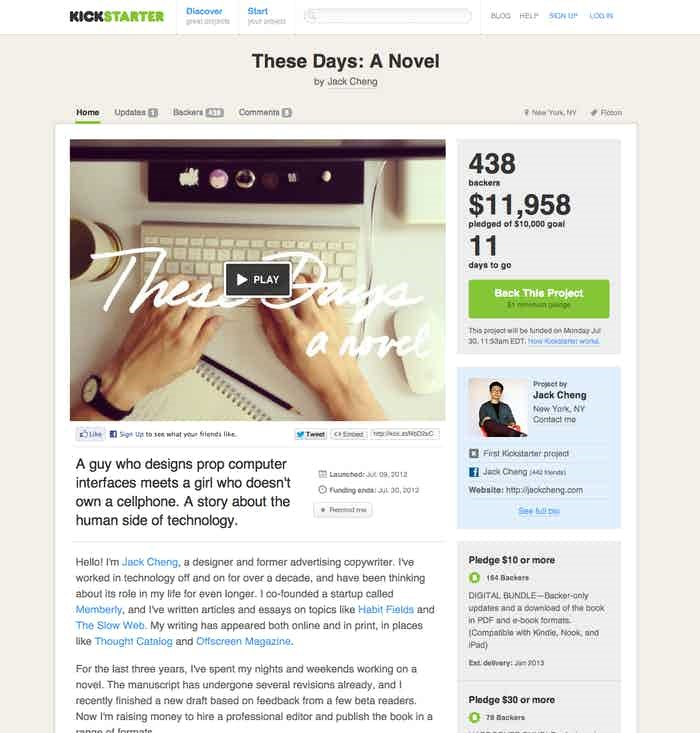
\includegraphics[width=0.70\textwidth]{2/figures/kickstarter_project.jpg}
		\caption[Ejemplo de proyecto vigente en Kickstarter]{Ejemplo de proyecto vigente en Kickstarter.\\
			Fuente: \cite{cr_perry2012kickstarterproject}. \textit{The New Project Page}.}
		\label{2:fig51}
	\end{center}
\end{figure}

\subsection{Proyecto}
Un proyecto es un esfuerzo temporal que se lleva a cabo para crear un producto, servicio o resultado único. La naturaleza temporal de los proyectos indica un principio y un final definidos, y que el propósito se alcanza cuando se logran los objetivos del proyecto o cuando este es terminado por no cumplir sus objetivos, o cuando ya no existe la necesidad inicial que dio origen al mismo \parencite{bk_pmi2017pmbokguide}.

A partir de este concepto enunciado por el PMI, se entiende que un proyecto parte de una idea que un individuo o conjunto de individuos tienen en mente para convertirla en realidad con el fin de responder a una necesidad.

En Kickstarter, los proyectos que pueden ser financiados deben pertenecer a las siguientes categorías: Arte, Cómics, Artesanías, Baile, Diseño, Moda, Cine y vídeo, Comida, Juegos, Periodismo, Música, Fotografía, Publicaciones, Tecnología, y Teatro. Cualquier tipo de persona puede contribuir al mismo desde ser patrocinadores hasta formar parte de las principales referencias \parencite{cr_kickstarter_learn}.

Dentro de las normas internas de la plataforma para la creación de proyectos se especifica que cada proyecto debe resultar ser totalmente nuevo, original e innovador que pueda ser compartido con el público, así como haber sido presentados de forma honesta y clara. En adición a esto, también se menciona que las recaudaciones que se darán no podrán ser otorgadas a obras benéficas sino cumplir con el objetivo de llevar a cabo el proyecto planteado, al igual que está prohibido asimismo del ofrecimiento de incentivos financieros como resultado \parencite{cr_kickstarter_rules}.


\subsection{Campaña}
Una campaña puede abarcar diversos términos si es que se busca su concepto en fuentes confiables como la Real Academia Española debido al alcance y empleabilidad del mismo. El significado más próximo que la RAE enuncia sobre campaña es la de un “conjunto de actos o esfuerzos de índole diversa que se aplican a conseguir un fin determinado” \parencite{gl_rae}. Para el actual contexto, el término se refiere específicamente a la campaña publicitaria, la cual se define como una estrategia diseñada y ejecutada en diferentes medios para obtener objetivos de notoriedad, ventas y comunicación de una determinada marca o producto a través del uso de la publicidad \parencite{tec_cyberclic_campaign}.

En la plataforma de Kickstarter, existen personas que tienen ideas y proyectos en mente, buscando financiarlos en el sitio web. Para lograr su objetivo y siguiendo la regla del “todo o nada”, estos individuos realizan eventos de promoción para atraer entre personas conocidas suyas y cibernautas en general. A esta serie de eventos de promoción se le conoce como campañas. Las campañas exitosas se basan en que un determinado proyecto alcanza a ser financiado en el tiempo estimado gracias a algunas de las siguientes características \parencite{cr_kickstarter_intro}:

\begin{itemize}
	\item Logran ser claros y concisos sobre lo que su proyecto busca alcanzar al ser financiado. Se definen bien las características del proyecto mediante detalles en la descripción, videos e imágenes precisas.
	\item Indican los beneficios y recompensas que los patrocinadores obtendrán si es que la campaña es exitosa y el proyecto se financia.
	\item Atrae e interactúa con una gran cantidad de público, manteniendo constante comunicación acerca de actualizaciones y novedades de la campaña y resolviendo dudas que puedan darse.
	\item Se estiman costos de manera eficiente que pueden ser solventados para cubrir más allá del proyecto una vez financiado, incluido los que se originan para la entrega del producto a los patrocinadores. Se logra convencerlos.
\end{itemize}

El autor \cite{cr_yu2017kickstarter_course} también complementa lo anterior con las siguientes estrategias para empezar a realizar la campaña:

\begin{itemize}
	\item Además de estimar los costos, se debe contar con un buffer en caso ocurra un imprevisto. Se puede determinar la meta a través de la fórmula (Gastos + Buffer) x Alcance.
	\item Un proyecto con video tiene 50\% de chance de tener éxito. El promedio de su duración debería ser de 3.38 minutos, aunque el público presta más atención hacia aquellos que duran poco. El vídeo debe contener y responder las siguientes preguntas:
	\begin{itemize}
		\item ¿Qué hace memorable al proyecto?
		\item ¿Cómo se verá el proyecto?
		\item ¿Por qué se está creando el producto?
		\item ¿Por qué se necesita?
		\item ¿Por qué es importante que el proyecto exista?
		\item ¿Por qué se debe ser creador?
		\item ¿Por qué deben escoger la compañía?
		\item ¿Cómo se proveerá una solución?
		\item ¿Cómo funciona la solución?
	\end{itemize}
	Es importante destacar las estadísticas del problema que se piensa resolver al inicio del video ya que el primer minuto resulta ser el lapso de tiempo que más capta la atención del público. Se recomienda también tener buen audio e iluminación.
	\item La descripción deberá ser un resumen de los puntos más relevantes del producto. Se debe mencionar una breve introducción del proyecto, cómo funciona, quiénes son el público objetivo, el proceso que se siguió en el desarrollo, detalles y especificaciones, y un cronograma e hitos.
	\item Las imágenes deben comunicar cómo lucirá el proyecto. Esta prueba convencerá a más de una persona en querer invertir en el proyecto. Las imágenes a veces atraen más a las personas que no gustan leer la descripción completa del proyecto.
	\item Al basarse en un modelo de crowdfunding en recompensas, los patrocinadores esperan un beneficio por parte del proyecto una vez este logre alcanzar su financiamiento. El número ideal de recompensas puede ser entre 5 y 7. Una recompensa en promedio de \$100 es la que genera más dinero. Las recompensas pueden ser de cuatro tipos: el producto en sí mismo entregado hacia los patrocinadores antes que este salga al mercado, reconocimientos en la página web y acceso hacia actualizaciones, recuerdos y certificados de membresía, y nuevas experiencias como visita a los desarrolladores en sus estudios.
\end{itemize}

Adicional a estos puntos, se descubrió en una investigación con más de 27 mil proyectos en Kickstarter que, a pesar que el número de proyectos iniciados por varones es dos veces más que de mujeres, el ratio de éxito de financiamiento es mayor en ellas. Esto debido a que las creadoras, en general, establecen objetivos más realísticos y con un tiempo límite más bajo para cumplir sus objetivos, transmitiendo así calidad y confianza para que los inversores actúen más rápido \parencite{cr_ullah2020crowdfunding}.

Otro factor clave es el rol importante de los patrocinadores en el éxito de un proyecto financiado. Sus principales motivaciones vienen dadas a factores como las recompensas por el aporte económico al proyecto, el nivel de innovación que este ofrece, la participación social que se logre captar, entre otros. Podrían clasificarse estas motivaciones en 6 grupos: interés, diversión, filantropía, recompensa, relación y reconocimiento. El resultado, 4 tipos de patrocinadores: los angelicales (donantes tradicionales), cazadores de recompensas (inversores del mercado), ávidos fanáticos (apasionados como los miembros de una comunidad de marca) y ermitaños de buen gusto (fanáticos discretos pero entusiastas) \parencite{cr_tung2019backers}.